\doublespacing
\chap{Experiments and Results}
\label{chap:EnR}

\section{Introduction}

In this chapter, we look at the implementation perspective of the whole system. We also look at the two dataset we used and the results obtained from them. 

\section{Implementation Details}
To implement the conditional generative adversarial network we used Tensorflow \cite{tensorflow2015-whitepaper} with Kera \cite{keras} as our framework. These libraries not only provide enough support for our approach but also have very optimized code to run on powerful GPUs. The structure of the generator and discriminator are described in \cref{Generator-Activation} and \cref{Discriminator-Table}.
\begin{table}[ht]
\centering
\caption{Generator Architecture Specification}
\label{Generator-Activation}
\begin{tabular}{llll}
Operation       & Stride & Features & Activation \\
Merge Input     & -      & -        & -          \\
Dense layer     & -      & -        & Sigmoid    \\
Deconvolution 1 & 5 * 5  & 512      & RELU       \\
Deconvolution 2 & 5 * 5    & 256      & RELU       \\
Deconvolution 3 & 5 * 5   & 128      & RELU       \\
Deconvolution 4 & 5 * 5   & 64       & RELU       \\
Deconvolution 5 & 5 * 5  & 3        & Tanh      
\end{tabular}
\end{table}
\begin{table}[ht]
\centering
\caption{Discriminator Architecture Specification}
\label{Discriminator-Table}
\begin{tabular}{llll}
Operation     & Stride & Features & Activation \\
Convolution 1 & 5 * 5  & 64       & Leaky RELU \\
Convolution 2 & 5*5    & 128      & LeakyRELU  \\
Convolution 3 & 5 *5   & 256      & LeakyRELU  \\
Convolution 4 & 5 *5   & 512      & LeakyRELU  \\
Convolution 5 & 5 * 5  & 1        & Softmax    \\
Convolution 5 & 5*5    & 18       & Sigmoid   
\end{tabular}
\end{table}
\section{Training}
Since the discriminator was weak, before actual training we trained the discriminator in two steps. Firstly, we added a conditional vector to its input and removed the classification output of it. Then we trained the discriminator with real images with incorrect labels to classify as fake images. Later, to the original discriminator we copied the weights from the previous, training and trained again on real images to classify them into the particular class.  


In the \cref{fig:train-celeba}, we can look at the training losses for the generator and the discriminator. As we can observe after pre-training a GAN, we are able to reach an equilibrium loss for both generator and discriminator at around epoch 30. If we also look at graph closely, in starting epoch the generator and discriminator have a huge loss gap as we are playing minmax game and as the we progress the gap in looses starts to shrink. The \cref{fig:train-mnist} shows the loss of the generator and discriminator when trained using MNIST \cite{MNIST} images. The number of epochs required by MNIST is very less as compared to celeba, as details required to generate a face are more complex as compared to digits.

\begin{figure}[H]
  \centering
    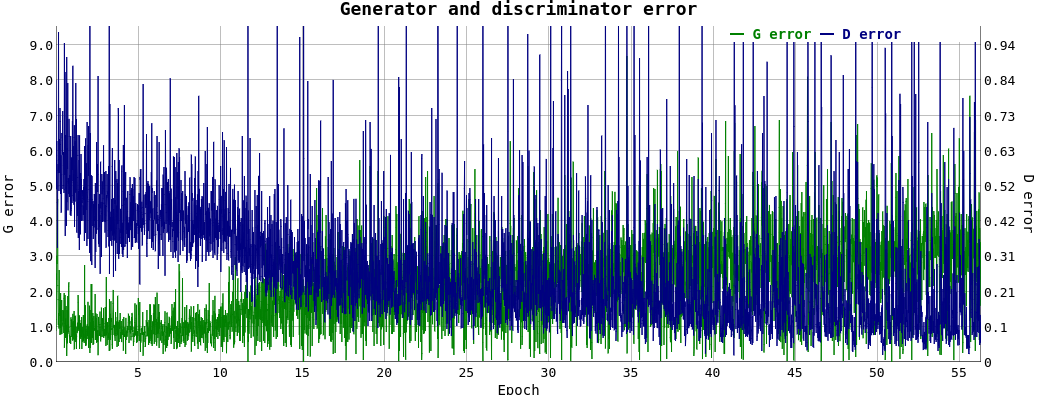
\includegraphics[scale=.4, angle=0]{Files/Training-2.png}
    \caption[Generator Discrminator Loss for Celeba dataset]{}
    \label{fig:train-celeba}
\end{figure}

\begin{figure}[H]
  \centering
    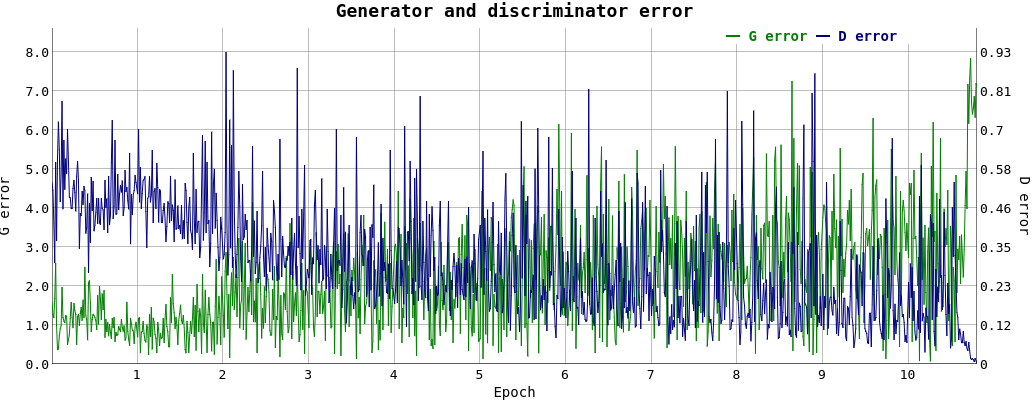
\includegraphics[scale=.4, angle=0]{Files/MNIST-GAN.png}
    \caption[Generator Discrminator Loss for MNIST dataset]{}
    \label{fig:train-mnist}
\end{figure}
\section{Dataset}
\subsection{CelebA}
The CelebFaces Attributes dataset (CelebA) \cite{celeba} contains 202599 face images of celebrities. As some of the categories are very infrequent , so we removed certain categories from our training. The distribution of the overall dataset is shown in \cref{fig:celeba}. As part of preprocessing, we crop the pre-aligned images to $64 \times 64$. The reason for cropping the images is to focus on faces in the images and remove as much as background possible.


\begin{figure}[H]
  \centering
    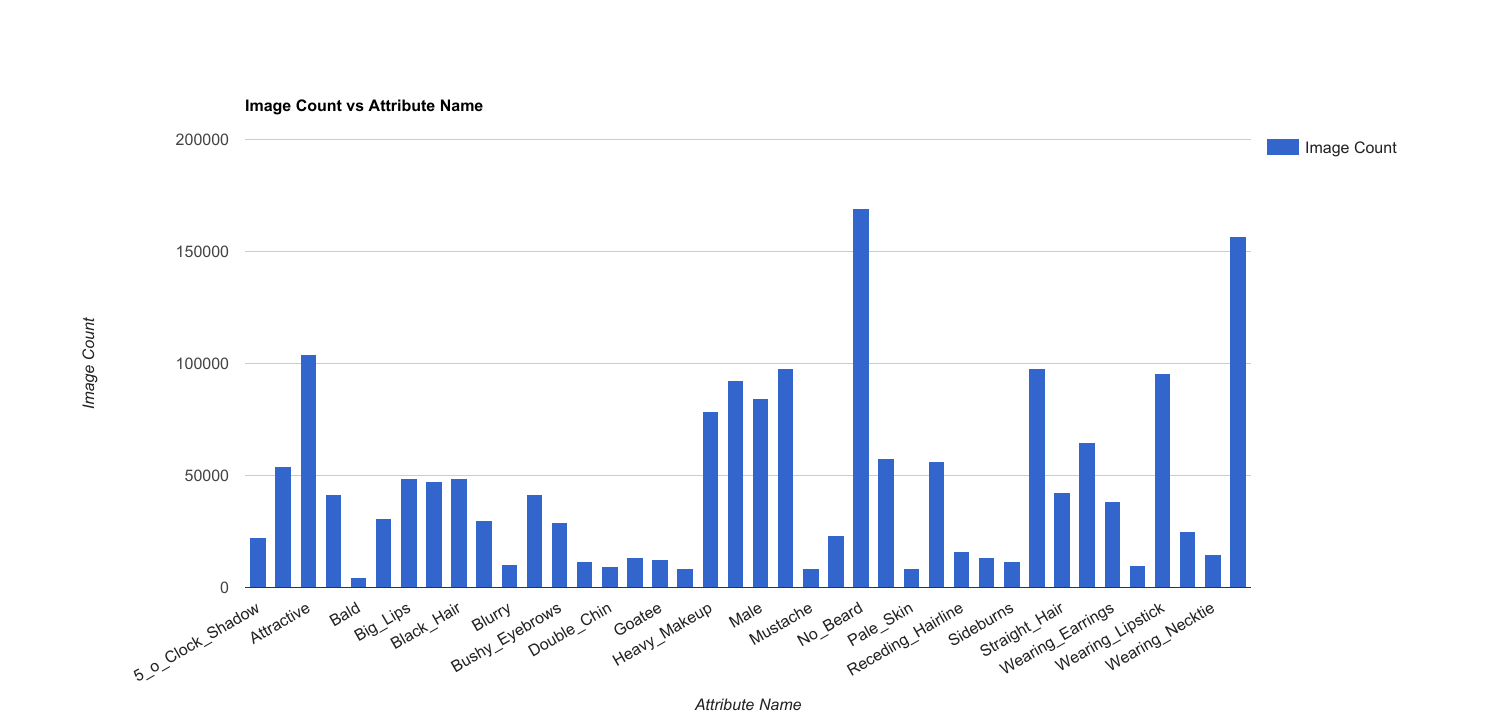
\includegraphics[scale=.3, angle=0]{Files/celeba-visualize.png}
    \caption[Generator Architecture]{Generator Architecture\cite{DCGAN}}
    \label{fig:celeba}
\end{figure}
%\subsection{CIFAR-10}

\subsection{MNIST}
MNIST \cite{MNIST} dataset is a standard image processing dataset. This dataset contains 60000 labeled images of digits from 0 to 9. This dataset helps in validating the models correctness in a very short time. Since neural  networks take lot of time to converge, if we have some issue with our implementation or logic then we can debug in a much shorter amount of time using this dataset.

\section{Results}

Once the generator has been trained, we look at the images being generated by our generator by passing some random noise (z) along with the conditional vector. We can see in \cref{Celeb-a} the various different category facial images being drawn by our generator. There were several categories as shown in \cref{U-celeb-a} for which generator was unsuccessful in getting desired facial attributes. Similarly, we generated different kind of digits from the MNIST trained generator as shown in \cref{MNIST-Result}. Since the MNIST dataset does not involve much complexity, there were very less unsuccessful results when generating specific digits.

  

\begin{table}[ht]
\centering
\caption{Successfully Generated Celebrity Images}
\label{Celeb-a}
\begin{tabular}{|llllll|}
\hline
Bald & 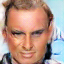
\includegraphics[width=1.69cm, height=1.69cm]{Files/images/images1/image100.png}  &
\includegraphics[width=1.69cm, height=1.69cm]{Files/images/images1/image2.png}   & 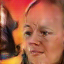
\includegraphics[width=1.69cm, height=1.69cm]{Files/images/images1/image3.png}  & 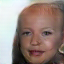
\includegraphics[width=1.69cm, height=1.69cm]{Files/images/images1/image52.png}  & 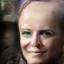
\includegraphics[width=1.69cm, height=1.69cm]{Files/images/images1/image68.png} \\ \hline


Bangs & 
\includegraphics[width=1.69cm, height=1.69cm]{Files/images/images2/image74.png}  &
\includegraphics[width=1.69cm, height=1.69cm]{Files/images/images2/image9.png}   & 
\includegraphics[width=1.69cm, height=1.69cm]{Files/images/images2/image77.png}  & 
\includegraphics[width=1.69cm, height=1.69cm]{Files/images/images2/image79.png}  & 
\includegraphics[width=1.69cm, height=1.69cm]{Files/images/images2/image48.png} \\ \hline


Black Hair & 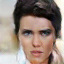
\includegraphics[width=1.69cm, height=1.69cm]{Files/images/images3/image94.png}  &
\includegraphics[width=1.69cm, height=1.69cm]{Files/images/images3/image60.png}   & 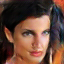
\includegraphics[width=1.69cm, height=1.69cm]{Files/images/images3/image56.png}  & 
\includegraphics[width=1.69cm, height=1.69cm]{Files/images/images3/image87.png}  & 
\includegraphics[width=1.69cm, height=1.69cm]{Files/images/images3/image76.png} \\ \hline


Blond & 
\includegraphics[width=1.69cm, height=1.69cm]{Files/images/images4/image86.png}  &
\includegraphics[width=1.69cm, height=1.69cm]{Files/images/images4/image64.png}   & 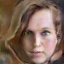
\includegraphics[width=1.69cm, height=1.69cm]{Files/images/images4/image91.png}  & 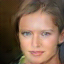
\includegraphics[width=1.69cm, height=1.69cm]{Files/images/images4/image5.png}  & 
\includegraphics[width=1.69cm, height=1.69cm]{Files/images/images4/image25.png} \\ \hline


Male & 
\includegraphics[width=1.69cm, height=1.69cm]{Files/images/images10/image12.png}  &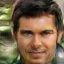
\includegraphics[width=1.69cm, height=1.69cm]{Files/images/images10/image32.png}   & 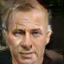
\includegraphics[width=1.69cm, height=1.69cm]{Files/images/images10/image19.png}  & 
\includegraphics[width=1.69cm, height=1.69cm]{Files/images/images10/image34.png}  & 
\includegraphics[width=1.69cm, height=1.69cm]{Files/images/images10/image55.png} \\ \hline

Mouth Open  & 
\includegraphics[width=1.69cm, height=1.69cm]{Files/images/images11/image70.png}  &
\includegraphics[width=1.69cm, height=1.69cm]{Files/images/images11/image69.png}   & 
\includegraphics[width=1.69cm, height=1.69cm]{Files/images/images11/image65.png}  & 
\includegraphics[width=1.69cm, height=1.69cm]{Files/images/images11/image37.png}  & 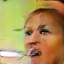
\includegraphics[width=1.69cm, height=1.69cm]{Files/images/images11/image7.png} \\ \hline

Smiling  & 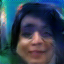
\includegraphics[width=1.69cm, height=1.69cm]{Files/images/images15/image70.png}  &
\includegraphics[width=1.69cm, height=1.69cm]{Files/images/images15/image7.png}   & 
\includegraphics[width=1.69cm, height=1.69cm]{Files/images/images15/image47.png}  & 
\includegraphics[width=1.69cm, height=1.69cm]{Files/images/images15/image37.png}  & 
\includegraphics[width=1.69cm, height=1.69cm]{Files/images/images15/image76.png} \\ \hline

Eye Glasses  & 
\includegraphics[width=1.69cm, height=1.69cm]{Files/images/images7/image79.png}  &
\includegraphics[width=1.69cm, height=1.69cm]{Files/images/images7/image4.png}   & 
\includegraphics[width=1.69cm, height=1.69cm]{Files/images/images7/image27.png}  & 
\includegraphics[width=1.69cm, height=1.69cm]{Files/images/images7/image25.png}  & 
\includegraphics[width=1.69cm, height=1.69cm]{Files/images/images7/image67.png} \\ \hline

Eye Glasses  & 
\includegraphics[width=1.69cm, height=1.69cm]{Files/images/images7/image79.png}  &
\includegraphics[width=1.69cm, height=1.69cm]{Files/images/images7/image4.png}   & 
\includegraphics[width=1.69cm, height=1.69cm]{Files/images/images7/image27.png}  & 
\includegraphics[width=1.69cm, height=1.69cm]{Files/images/images7/image25.png}  & 
\includegraphics[width=1.69cm, height=1.69cm]{Files/images/images7/image67.png} \\ \hline
\end{tabular}
\end{table}

\begin{table}[H]
\centering
\caption{Unsuccessful Generated Celebrity Images}
\label{U-celeb-a}
\begin{tabular}{|llllll|}
\hline
Wearing Hat & 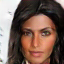
\includegraphics[width=1.69cm, height=1.69cm]{Files/images/images18/image1.png}  &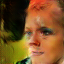
\includegraphics[width=1.69cm, height=1.69cm]{Files/images/images18/image2.png}   & \includegraphics[width=1.69cm, height=1.69cm]{Files/images/images18/image3.png}  & \includegraphics[width=1.69cm, height=1.69cm]{Files/images/images18/image52.png}  & \includegraphics[width=1.69cm, height=1.69cm]{Files/images/images18/image68.png} \\ \hline


Wavy Hair & \includegraphics[width=1.69cm, height=1.69cm]{Files/images/images17/image1.png}  &\includegraphics[width=1.69cm, height=1.69cm]{Files/images/images17/image2.png}   & \includegraphics[width=1.69cm, height=1.69cm]{Files/images/images17/image3.png}  & \includegraphics[width=1.69cm, height=1.69cm]{Files/images/images17/image52.png}  & \includegraphics[width=1.69cm, height=1.69cm]{Files/images/images17/image68.png} \\ \hline

Receding Hairline & \includegraphics[width=1.69cm, height=1.69cm]{Files/images/images14/image1.png}  &\includegraphics[width=1.69cm, height=1.69cm]{Files/images/images14/image2.png}   & \includegraphics[width=1.69cm, height=1.69cm]{Files/images/images14/image3.png}  & \includegraphics[width=1.69cm, height=1.69cm]{Files/images/images14/image52.png}  & \includegraphics[width=1.69cm, height=1.69cm]{Files/images/images14/image68.png} \\ \hline


\end{tabular}
\end{table}

\begin{table}[H]
\centering
\caption{Successfully Generated MNIST Images}
\label{MNIST-Result}
\begin{tabular}{|llllll|}
\hline
0 & \includegraphics[width=1.69cm, height=1.69cm]{Files/MNIST/0-0.png}  &\includegraphics[width=1.69cm,  height=1.69cm]{Files/MNIST/1-2.png}   & \includegraphics[width=1.69cm, height=1.69cm]{Files/MNIST/2-4.png}  & \includegraphics[width=1.69cm, height=1.69cm]{Files/MNIST/5-0.png}  & \includegraphics[width=1.69cm, height=1.69cm]{Files/MNIST/6-2.png} \\ \hline

1 & \includegraphics[width=1.69cm, height=1.69cm]{Files/MNIST/0-1.png}  &\includegraphics[width=1.69cm, height=1.69cm]{Files/MNIST/1-3.png}   & \includegraphics[width=1.69cm, height=1.69cm]{Files/MNIST/2-5.png}  & \includegraphics[width=1.69cm, height=1.69cm]{Files/MNIST/5-1.png}  & \includegraphics[width=1.69cm, height=1.69cm]{Files/MNIST/7-5.png} \\ \hline

2 & \includegraphics[width=1.69cm, height=1.69cm]{Files/MNIST/0-2.png}  &\includegraphics[width=1.69cm, height=1.69cm]{Files/MNIST/1-4.png}   & \includegraphics[width=1.69cm, height=1.69cm]{Files/MNIST/2-6.png}  & \includegraphics[width=1.69cm, height=1.69cm]{Files/MNIST/5-2.png}  & \includegraphics[width=1.69cm, height=1.69cm]{Files/MNIST/6-4.png} \\ \hline

3 & \includegraphics[width=1.69cm, height=1.69cm]{Files/MNIST/0-3.png}  &\includegraphics[width=1.69cm, height=1.69cm]{Files/MNIST/1-5.png}   & \includegraphics[width=1.69cm, height=1.69cm]{Files/MNIST/2-7.png}  & \includegraphics[width=1.69cm, height=1.69cm]{Files/MNIST/5-3.png}  & \includegraphics[width=1.69cm, height=1.69cm]{Files/MNIST/6-5.png} \\ \hline

4 & \includegraphics[width=1.69cm, height=1.69cm]{Files/MNIST/0-4.png}  &\includegraphics[width=1.69cm, height=1.69cm]{Files/MNIST/1-6.png}   & \includegraphics[width=1.69cm, height=1.69cm]{Files/MNIST/3-0.png}  & \includegraphics[width=1.69cm, height=1.69cm]{Files/MNIST/5-4.png}  & \includegraphics[width=1.69cm, height=1.69cm]{Files/MNIST/6-6.png} \\ \hline

5 & \includegraphics[width=1.69cm, height=1.69cm]{Files/MNIST/0-5.png}  &\includegraphics[width=1.69cm, height=1.69cm]{Files/MNIST/1-7.png}   & \includegraphics[width=1.69cm, height=1.69cm]{Files/MNIST/3-1.png}  & \includegraphics[width=1.69cm, height=1.69cm]{Files/MNIST/5-5.png}  & \includegraphics[width=1.69cm, height=1.69cm]{Files/MNIST/6-7.png} \\ \hline

6 & \includegraphics[width=1.69cm, height=1.69cm]{Files/MNIST/0-6.png}  &\includegraphics[width=1.69cm, height=1.69cm]{Files/MNIST/2-0.png}   & \includegraphics[width=1.69cm, height=1.69cm]{Files/MNIST/3-2.png}  & \includegraphics[width=1.69cm, height=1.69cm]{Files/MNIST/5-6.png}  & \includegraphics[width=1.69cm, height=1.69cm]{Files/MNIST/7-0.png} \\ \hline

7 & \includegraphics[width=1.69cm, height=1.69cm]{Files/MNIST/0-7.png}  &\includegraphics[width=1.69cm, height=1.69cm]{Files/MNIST/2-1.png}   & \includegraphics[width=1.69cm, height=1.69cm]{Files/MNIST/3-3.png}  & \includegraphics[width=1.69cm, height=1.69cm]{Files/MNIST/4-5.png}  & \includegraphics[width=1.69cm, height=1.69cm]{Files/MNIST/5-7.png} \\ \hline

8 & \includegraphics[width=1.69cm, height=1.69cm]{Files/MNIST/1-0.png}  &\includegraphics[width=1.69cm, height=1.69cm]{Files/MNIST/2-2.png}   & \includegraphics[width=1.69cm, height=1.69cm]{Files/MNIST/3-4.png}  & \includegraphics[width=1.69cm, height=1.69cm]{Files/MNIST/4-6.png}  & \includegraphics[width=1.69cm, height=1.69cm]{Files/MNIST/7-2.png} \\ \hline

9 & \includegraphics[width=1.69cm, height=1.69cm]{Files/MNIST/1-1.png}  &\includegraphics[width=1.69cm, height=1.69cm]{Files/MNIST/2-3.png}   & \includegraphics[width=1.69cm, height=1.69cm]{Files/MNIST/4-7.png}  & \includegraphics[width=1.69cm, height=1.69cm]{Files/MNIST/6-1.png}  & \includegraphics[width=1.69cm, height=1.69cm]{Files/MNIST/7-3.png} \\ \hline

\end{tabular}
\end{table}



\section{Evaluation}

It is very challenging to evaluate the performance of GAN networks as there has been no comparable method to judge the quality of images being produced.  To evaluate the performance of celebA \cite{celeba} dataset, we use the same discriminator and we train it over the real images dataset. Later we passed 100 generated images from each category to this CNN to obtain a mean accuracy of 85.23\%. We also ran text over Microsoft's Vision API \cite{Microsoft}, where we passed 1000 facial images for which it was able to detect faces with 96.88\%. 